% Options for packages loaded elsewhere
% Options for packages loaded elsewhere
\PassOptionsToPackage{unicode}{hyperref}
\PassOptionsToPackage{hyphens}{url}
\PassOptionsToPackage{dvipsnames,svgnames,x11names}{xcolor}
%
\documentclass[
  spanish,
  spanish,
  es-tabla,
  twocolumn]{llncs}
\usepackage{xcolor}
\usepackage{amsmath,amssymb}
\setcounter{secnumdepth}{-\maxdimen} % remove section numbering
\usepackage{iftex}
\ifPDFTeX
  \usepackage[T1]{fontenc}
  \usepackage[utf8]{inputenc}
  \usepackage{textcomp} % provide euro and other symbols
\else % if luatex or xetex
  \usepackage{unicode-math} % this also loads fontspec
  \defaultfontfeatures{Scale=MatchLowercase}
  \defaultfontfeatures[\rmfamily]{Ligatures=TeX,Scale=1}
\fi
\usepackage{lmodern}
\ifPDFTeX\else
  % xetex/luatex font selection
\fi
% Use upquote if available, for straight quotes in verbatim environments
\IfFileExists{upquote.sty}{\usepackage{upquote}}{}
\IfFileExists{microtype.sty}{% use microtype if available
  \usepackage[]{microtype}
  \UseMicrotypeSet[protrusion]{basicmath} % disable protrusion for tt fonts
}{}
\makeatletter
\@ifundefined{KOMAClassName}{% if non-KOMA class
  \IfFileExists{parskip.sty}{%
    \usepackage{parskip}
  }{% else
    \setlength{\parindent}{0pt}
    \setlength{\parskip}{6pt plus 2pt minus 1pt}}
}{% if KOMA class
  \KOMAoptions{parskip=half}}
\makeatother
% Make \paragraph and \subparagraph free-standing
\makeatletter
\ifx\paragraph\undefined\else
  \let\oldparagraph\paragraph
  \renewcommand{\paragraph}{
    \@ifstar
      \xxxParagraphStar
      \xxxParagraphNoStar
  }
  \newcommand{\xxxParagraphStar}[1]{\oldparagraph*{#1}\mbox{}}
  \newcommand{\xxxParagraphNoStar}[1]{\oldparagraph{#1}\mbox{}}
\fi
\ifx\subparagraph\undefined\else
  \let\oldsubparagraph\subparagraph
  \renewcommand{\subparagraph}{
    \@ifstar
      \xxxSubParagraphStar
      \xxxSubParagraphNoStar
  }
  \newcommand{\xxxSubParagraphStar}[1]{\oldsubparagraph*{#1}\mbox{}}
  \newcommand{\xxxSubParagraphNoStar}[1]{\oldsubparagraph{#1}\mbox{}}
\fi
\makeatother


\usepackage{longtable,booktabs,array}
\newcounter{none} % for unnumbered tables
\usepackage{calc} % for calculating minipage widths
% Correct order of tables after \paragraph or \subparagraph
\usepackage{etoolbox}
\makeatletter
\patchcmd\longtable{\par}{\if@noskipsec\mbox{}\fi\par}{}{}
\makeatother
% Allow footnotes in longtable head/foot
\IfFileExists{footnotehyper.sty}{\usepackage{footnotehyper}}{\usepackage{footnote}}
\makesavenoteenv{longtable}
\usepackage{graphicx}
\makeatletter
\newsavebox\pandoc@box
\newcommand*\pandocbounded[1]{% scales image to fit in text height/width
  \sbox\pandoc@box{#1}%
  \Gscale@div\@tempa{\textheight}{\dimexpr\ht\pandoc@box+\dp\pandoc@box\relax}%
  \Gscale@div\@tempb{\linewidth}{\wd\pandoc@box}%
  \ifdim\@tempb\p@<\@tempa\p@\let\@tempa\@tempb\fi% select the smaller of both
  \ifdim\@tempa\p@<\p@\scalebox{\@tempa}{\usebox\pandoc@box}%
  \else\usebox{\pandoc@box}%
  \fi%
}
% Set default figure placement to htbp
\def\fps@figure{htbp}
\makeatother


% definitions for citeproc citations
\NewDocumentCommand\citeproctext{}{}
\NewDocumentCommand\citeproc{mm}{%
  \begingroup\def\citeproctext{#2}\cite{#1}\endgroup}
\makeatletter
 % allow citations to break across lines
 \let\@cite@ofmt\@firstofone
 % avoid brackets around text for \cite:
 \def\@biblabel#1{}
 \def\@cite#1#2{{#1\if@tempswa , #2\fi}}
\makeatother
\newlength{\cslhangindent}
\setlength{\cslhangindent}{1.5em}
\newlength{\csllabelwidth}
\setlength{\csllabelwidth}{3em}
\newenvironment{CSLReferences}[2] % #1 hanging-indent, #2 entry-spacing
 {\begin{list}{}{%
  \setlength{\itemindent}{0pt}
  \setlength{\leftmargin}{0pt}
  \setlength{\parsep}{0pt}
  % turn on hanging indent if param 1 is 1
  \ifodd #1
   \setlength{\leftmargin}{\cslhangindent}
   \setlength{\itemindent}{-1\cslhangindent}
  \fi
  % set entry spacing
  \setlength{\itemsep}{#2\baselineskip}}}
 {\end{list}}
\usepackage{calc}
\newcommand{\CSLBlock}[1]{\hfill\break\parbox[t]{\linewidth}{\strut\ignorespaces#1\strut}}
\newcommand{\CSLLeftMargin}[1]{\parbox[t]{\csllabelwidth}{\strut#1\strut}}
\newcommand{\CSLRightInline}[1]{\parbox[t]{\linewidth - \csllabelwidth}{\strut#1\strut}}
\newcommand{\CSLIndent}[1]{\hspace{\cslhangindent}#1}

\ifLuaTeX
\usepackage[bidi=basic,shorthands=off]{babel}
\else
\usepackage[bidi=default,shorthands=off]{babel}
\fi
\ifLuaTeX
  \usepackage{selnolig} % disable illegal ligatures
\fi


\setlength{\emergencystretch}{3em} % prevent overfull lines

\providecommand{\tightlist}{%
  \setlength{\itemsep}{0pt}\setlength{\parskip}{0pt}}



 


\institute{Escuela Politécnica Nacional --- Facultad de Ingeniería de Sistemas}
\setlength{\parskip}{0.5em}
\setlength{\parindent}{0pt}
\makeatletter
\@ifpackageloaded{caption}{}{\usepackage{caption}}
\AtBeginDocument{%
\ifdefined\contentsname
  \renewcommand*\contentsname{Tabla de contenidos}
\else
  \newcommand\contentsname{Tabla de contenidos}
\fi
\ifdefined\listfigurename
  \renewcommand*\listfigurename{Listado de Figuras}
\else
  \newcommand\listfigurename{Listado de Figuras}
\fi
\ifdefined\listtablename
  \renewcommand*\listtablename{Listado de Tablas}
\else
  \newcommand\listtablename{Listado de Tablas}
\fi
\ifdefined\figurename
  \renewcommand*\figurename{Figura}
\else
  \newcommand\figurename{Figura}
\fi
\ifdefined\tablename
  \renewcommand*\tablename{Tabla}
\else
  \newcommand\tablename{Tabla}
\fi
}
\@ifpackageloaded{float}{}{\usepackage{float}}
\floatstyle{ruled}
\@ifundefined{c@chapter}{\newfloat{codelisting}{h}{lop}}{\newfloat{codelisting}{h}{lop}[chapter]}
\floatname{codelisting}{Listado}
\newcommand*\listoflistings{\listof{codelisting}{Listado de Listados}}
\makeatother
\makeatletter
\makeatother
\makeatletter
\@ifpackageloaded{caption}{}{\usepackage{caption}}
\@ifpackageloaded{subcaption}{}{\usepackage{subcaption}}
\makeatother
\usepackage{bookmark}
\IfFileExists{xurl.sty}{\usepackage{xurl}}{} % add URL line breaks if available
\urlstyle{same}
\hypersetup{
  pdftitle={Tarea Grupal DG\_2},
  pdfauthor={Justin Guevara; Jair Lezcano; Jhosua Saa},
  pdflang={es},
  colorlinks=true,
  linkcolor={blue},
  filecolor={Maroon},
  citecolor={Blue},
  urlcolor={Blue},
  pdfcreator={LaTeX via pandoc}}


\title{Tarea Grupal DG\_2}
\usepackage{etoolbox}
\makeatletter
\providecommand{\subtitle}[1]{% add subtitle to \maketitle
  \apptocmd{\@title}{\par {\large #1 \par}}{}{}
}
\makeatother
\subtitle{Implementación y optimización de un agente reactivo con
memoria en un entorno bidimensional}
\author{Justin Guevara \and Jair Lezcano \and Jhosua Saa}
\date{}
\begin{document}
\maketitle


\textbf{Enlace al repositorio de GitHub}:
\url{https://github.com/JUSTAILS/IA---GRUPO-3}

\subsection{Objetivos}\label{objetivos}

\subsubsection{General}\label{general}

Implementar un agente reactivo simple con memoria en un entorno
bidimensional para mejorar la eficiencia en la limpieza y el consumo
energético en comparación con una arquitectura básica sin estado.

\subsubsection{Específicos}\label{especuxedficos}

\begin{itemize}
\tightlist
\item
  Analizar las limitaciones y la ineficiencia de un agente reactivo
  simple básico mediante la ejecución de simulaciones en el entorno de
  prueba.
\item
  Diseñar una estructura de memoria interna y un patrón de barrido
  sistemático que permita al agente registrar celdas visitadas y evitar
  movimientos redundantes.
\item
  Incorporar un mecanismo de parada explícita y métricas de rendimiento
  para evaluar cuantitativamente la mejora en la autonomía y el consumo
  energético del agente.
\end{itemize}

\subsection{Introducción}\label{introducciuxf3n}

Un agente inteligente es cualquier entidad capaz de percibir su entorno
a través de sensores y actuar sobre él mediante actuadores {[}1{]}. Los
agentes reactivos simples representan la arquitectura de control más
elemental, ya que seleccionan sus acciones únicamente en función de la
percepción del estado actual, omitiendo cualquier tipo de historial o
memoria de percepciones pasadas. Aunque esta arquitectura destaca por su
bajo costo computacional y rapidez de respuesta, presenta limitaciones
severas en entornos complejos o de recursos finitos {[}2{]}. Cuando un
entorno exige cobertura completa, la ausencia de un estado interno
provoca comportamientos erráticos, visitas redundantes y un consumo
ineficiente de energía. El propósito de este trabajo es analizar las
ineficiencias de un agente reactivo simple básico, rediseñar su
arquitectura incorporando un estado interno de memoria de visitas y
evaluar cuantitativamente la mejora en el rendimiento mediante la
métrica PEAS.

\subsection{Especificación PEAS del agente y
entorno}\label{especificaciuxf3n-peas-del-agente-y-entorno}

La especificación PEAS (Rendimiento, Entorno, Actuadores, Sensores)
define formalmente el problema y establece las capacidades reales del
agente dentro de las especificaciones de software implementadas {[}1{]}.
A diferencia de enfoques más complejos, la arquitectura de este agente
se mantiene estrictamente fiel a una percepción local, lo que se refleja
directamente en cada componente del modelo. En cuanto al rendimiento,
este se evalúa maximizando el número de celdas limpias y procurando
reducir el consumo energético medido a través de los pasos tomados por
el agente mientras intenta limpiar la mayor cantidad de celdas sucias.
Asimismo, otra forma de evaluación consiste en establecer una relación
entre las casillas limpiadas y los pasos dados por el agente. Estas
mediciones permiten observar si el agente opera de manera eficiente y
cumple con su meta adecuadamente. Todo esto toma en cuenta un entorno
representado por una cuadrícula bidimensional cuyas celdas adoptan
valores de 1 o 0 para indicar si están sucias o limpias,
respectivamente, situando inicialmente al agente en una posición
aleatoria dentro de la matriz. Con respecto a los actuadores, el agente
dispone de acciones para interactuar con el entorno, las cuales son:
limpiar la celda actual mediante la instrucción Suck, realizar
desplazamientos direccionales válidos dentro de los límites de la matriz
(Up, Down, Left, Right) y la condición de parada o finalización (Stop).
Frente a los sensores, se toma en cuenta que el agente no cuenta con una
cámara cenital, un visor global ni ningún mecanismo externo que le
indique cuántas celdas están sucias en todo el mapa de manera
simultánea. Sus sensores se limitan únicamente a percibir su coordenada
actual y el estado de limpieza exacto de la casilla específica en la que
se encuentra parado en ese instante. Por esta razón, el agente no conoce
el estado global de antemano, y cualquier noción del entorno debe ser
descubierta de forma secuencial a través de su propio desplazamiento y
el uso de su memoria interna.

\subsection{Diagnóstico de ineficiencia del agente
base}\label{diagnuxf3stico-de-ineficiencia-del-agente-base}

Al analizar el código base del agente reactivo simple, se observa que
este opera únicamente con la percepción local inmediata de su celda
actual. Si la celda está sucia, ejecuta la acción de limpiar; si está
limpia, toma una decisión de movimiento al azar entre las direcciones
adyacentes válidas dentro de los límites de la cuadrícula. Esta
arquitectura básica genera consecuencias directas en el desempeño del
sistema. En primer lugar, se produce un movimiento a ciegas, ya que al
no almacenar información histórica de las celdas que ya recorrió, el
agente frecuentemente re-visita casillas que ya había limpiado
previamente, lo que desperdicia recursos y tiempo de ejecución. En
segundo lugar, existe una carencia de criterio de autonomía para
detenerse, debido a que el agente básico no puede determinar por sí
mismo cuándo el entorno está totalmente limpio utilizando únicamente sus
sensores locales básicos, provocando que siga moviéndose indefinidamente
a menos que un mecanismo externo detenga el ciclo por un límite de
pasos. Finalmente, se genera una alta ineficiencia energética, pues al
desplazarse de forma aleatoria sin un patrón de barrido ni memoria
interna, la cantidad de pasos necesarios para limpiar el entorno se
dispara, disminuyendo notablemente la métrica de rendimiento
establecida.

\subsection{Diseño y mejoras
implementadas}\label{diseuxf1o-y-mejoras-implementadas}

Al comparar la evolución del código base frente a la versión mejorada,
el cambio principal radica en que el agente dejó de operar en un bucle
cerrado sin control para optimizar sus decisiones según el entorno. Para
lograrlo, se amplió el sistema desde una cuadrícula estática de dos por
dos hacia un entorno escalable y parametrizable. Asimismo, se le asignó
una estructura de memoria interna que funciona como un registro de las
casillas ya recorridas. Gracias a esto, el agente filtra sus opciones de
movimiento: evalúa las direcciones adyacentes y descarta aquellas que ya
exploró, eliminando por completo los desplazamientos redundantes y el
desperdicio de recursos. Adicionalmente, se introdujo una acción de
parada mediante un comando explícito, evitando que el agente continúe
moviéndose indefinidamente cuando el entorno se encuentra completamente
limpio o cuando ya no existen celdas adyacentes pendientes de explorar.
Por último, se incorporaron fórmulas de rendimiento empírico que
permiten calcular matemáticamente la eficiencia del recorrido dividiendo
la suciedad inicial entre los pasos totales dados, junto con una métrica
orientada a evaluar los costos de desplazamiento. De esta manera, es
posible verificar objetivamente si el agente realiza movimientos
innecesarios.

\subsection{Resultados}\label{resultados}

Para evaluar de manera cuantitativa el comportamiento y la eficiencia
del agente, se llevaron a cabo pruebas experimentales estructuradas en
diez intentos por cada escenario de prueba: el agente base en una
cuadrícula de dos por dos, el agente modificado con memoria en la misma
dimensión, y el escalamiento del agente modificado a una cuadrícula de
tres por tres. Los registros numéricos detallados de estas ejecuciones
se presentan en la Figura 1, donde se recopilan las celdas sucias
iniciales, las celdas limpiadas, los pasos totales, el balance
energético y la relación de rendimiento.

\begin{figure}[H]

{\centering \pandocbounded{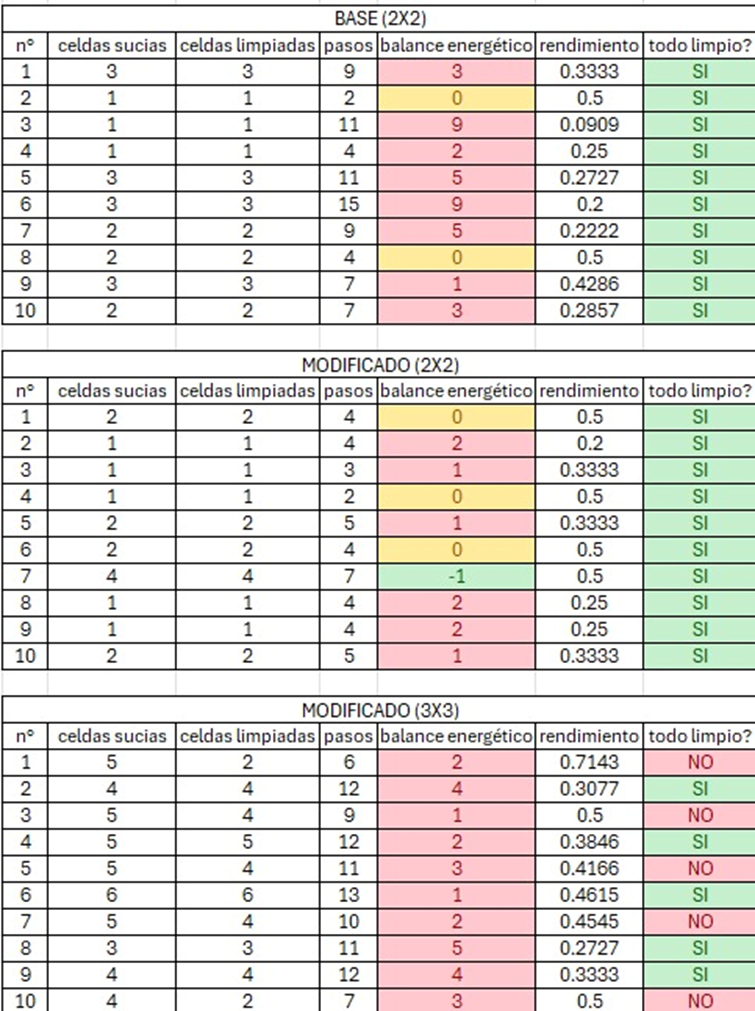
\includegraphics[keepaspectratio]{tablasComparativas.png}}

}

\caption{Tablas de comparación de resultados al analizar 10 intentos en
comparación del agente con código base y el modificado}

\end{figure}%

A partir de la observación de los datos tabulados en la Figura 1, se
identifica que el agente base en la cuadricula de dos por dos presenta
una alta dispersión en los pasos ejecutados, alcanzando hasta quince
pasos en el intento seis para limpiar tres casillas debido a su
exploración a ciegas. En contraste, los registros del agente modificado
en dos por dos muestran que los pasos se reducen a un rango de dos a
siete, optimizando el uso de recursos. Al analizar la relación entre los
pasos dados y las celdas limpiadas, se puede interpretar esta proporción
como un indicador de probabilidad o efectividad: el porcentaje de pasos
invertidos en relación con los cuadros limpiados refleja la probabilidad
de que el siguiente movimiento del agente lo conduzca de manera directa
a una casilla sucia para limpiarla, minimizando los desplazamientos al
vacío. Sin embargo, en el escenario escalado de tres por tres de la
tercera tabla en la Figura 1, aunque los pasos se mantienen controlados
entre seis y trece, la tasa de éxito en la limpieza total se divide al
cincuenta por ciento, evidenciando que la visión local pura del agente
puede provocar detenciones prematuras en mapas más grandes. Para
contrastar de forma visual las mejoras operativas obtenidas entre el
modelo base y el optimizado, se procesaron las métricas en las
representaciones graficas que se muestran en la Figura 1.

\begin{figure}[H]

{\centering \pandocbounded{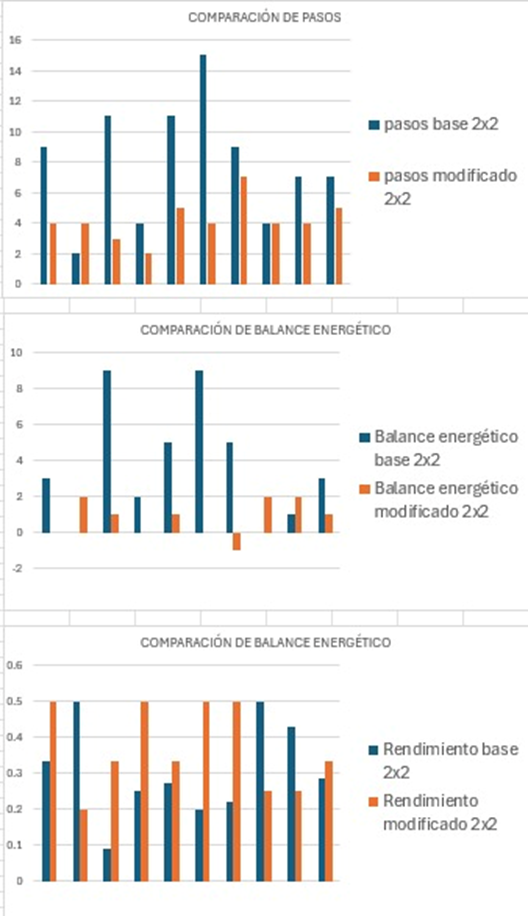
\includegraphics[keepaspectratio]{graficasRendimiento.png}}

}

\caption{Comparación gráfica de resultados entre el agente con código
base y el modificado.}

\end{figure}%

En la primera gráfica de la Figura 2, correspondiente a la comparación
de pasos, se observa claramente como las barras del agente base
experimentan picos elevados de hasta quince unidades, mientras que las
barras del agente modificado se mantienen estables y acotadas en la
parte inferior, confirmando que la memoria interna elimina los
recorridos redundantes. En la segunda gráfica de la Figura 2, que evalúa
el balance energético, el agente base acumula costos elevados que llegan
a nueve unidades de desperdicio por deambular sin rumbo, mientras que el
modelo modificado estabiliza su balance cerca de cero o registra valores
negativos en escenarios de mayor densidad, lo que demuestra una
reducción drástica del consumo energético. Finalmente, en la tercera
gráfica de la Figura 2 sobre el rendimiento, la relación entre el
trabajo realizado y los pasos tomados muestra que el agente modificado
sostiene picos constantes de hasta 0.5, validando que su probabilidad de
acierto y su eficiencia operativa mejoraron sustancialmente gracias al
patrón de barrido implementado.

\subsection{Conclusiones}\label{conclusiones}

\begin{itemize}
\tightlist
\item
  La arquitectura del agente reactivo simple basada únicamente en
  percepciones inmediatas presenta severas limitaciones operativas, como
  el deambuleo ciego y la ausencia de un criterio autónomo de parada, lo
  que genera un consumo innecesario de recursos y una baja eficiencia en
  tareas de cobertura y limpieza.
\item
  La implementación de una estructura de memoria interna y un patrón de
  barrido sistemático transforma radicalmente el comportamiento del
  agente, eliminando las trayectorias redundantes sobre casillas ya
  procesadas, reduciendo el costo energético y optimizando la relación
  entre los pasos dados y la probabilidad de acierto al encontrar celdas
  sucias.
\item
  La evaluación empírica en entornos escalados de mayor dimensión
  demuestra que, si bien la memoria local optimiza el rendimiento en
  espacios reducidos, la arquitectura basada en percepciones locales
  puras presenta limitaciones operativas. No obstante, estas
  deficiencias pueden mitigarse mejorando las capacidades de hardware
  del agente, permitiéndole integrar procesamiento avanzado para una
  toma de decisiones más robusta y dotando a sus actuadores de mayor
  precisión para interactuar de forma óptima con el entorno.
\end{itemize}

\subsection{Referencias}\label{referencias}

\protect\phantomsection\label{refs}
\begin{CSLReferences}{0}{0}
\bibitem[\citeproctext]{ref-russell2020artificial}
\CSLLeftMargin{{[}1{]} }%
\CSLRightInline{S. Russell y P. Norvig, \emph{Artificial Intelligence: A
Modern Approach}, 4th ed. Pearson, 2020.}

\bibitem[\citeproctext]{ref-wooldridge2009introduction}
\CSLLeftMargin{{[}2{]} }%
\CSLRightInline{M. Wooldridge, \emph{An Introduction to MultiAgent
Systems}, 2nd ed. Chichester, UK: John Wiley \& Sons, 2009.}

\end{CSLReferences}




\end{document}
